\FloatBarrier
\subsubsection{Computing evolution}
%\emph{
%Author(s):  S. Aoudia, L. Bosi, L. Storchi,  \\
%}
%\dots

Computing has made great strides in recent years in order to provide each year 
even more fast processors.
Since the invention of the integrated circuit in 1958, the number of 
transistors on a given chip double 
(roughly) every two years, as predicted by the first Moore's law \cite{MooreLaw}. 
This exponential growth has allowed computers to get 
both cheaper and more powerful at the same time (see Appendix \ref{sec:MLbox}
for more details).

%%%%%%%%%% Box MOORELAW

%\etbox{i}{box:MLbox}
%{Moores Law}
%{``Moore's Law is a violation of Murphy's Law. Everything gets better and 
%better''~\cite{MooresFrase2}
% this is how Gordon Moore
%commented the law, that bears his name, in 2005. Moore's law describes trend in 
%the history of computing
%hardware. The law has been originally thought to describes the number of 
%transistors that can be placed
%inexpensively on an integrated circuit. But now we see this law can be applied 
%also to the capabilities
%of many digital electronic devices, such as memory capacity, sensors and even 
%even the number and size
%of pixels in digital cameras. There are in fact many other laws related to the 
%Moore's one. Other laws
%prediction for example hard disk storage cost per unit of information, or 
%network capacity, or pixels
%per dollar, and more.
%\\[10pt]
%Gordon E. Moore formulated the law by a simple observation. In 1965 he noted 
%that number of components
%in integrated circuits had doubled every two years from the invention of the 
%integrated circuit in 1958. Thus, he predicted that the trend would continue 
%``for at least ten years''. Years after the law has been
%reformulated to take into account an higher growth, and the final formulation 
%state that integrated circuits
%would double in performance every 18 months. Thus ``Moore's first law predict'' 
%an exponential rates for the transistor counts in a microprocessor: $P_n = P_0 
%\cdot 2^n$, where $P_n$ is the predicted computer processing power in
%future years, $P_0$ is the actual computer processing power, and $n$ the number 
%of years divided by the doubling period, expressed in years. I.e.\ if we 
%consider the transistor count the doubling factor is 2 (every 2 years), while 
%if we consider the processors speed the doubling factor is 1.5 (every 18 
%months).
%\\[10pt]
%Moore's first law can be viewed just as an observation, but maybe there is even 
%more. Maybe behind
%it there is a more deeper law, a law driving evolution of information and 
%technology, of which the
%Moore's law is just a consequence. But up to now what it is clear is that this 
%law has been
%widely accepted, and is used as a goal for both marketing and engineering 
%departments of semiconductor
%manufacturers.
%}
%%%%%%%%%%%%%%%%%%%% ENDBOX MOORELAW

%%%%INSERT1
Quoting Moore's recent statment  issued during an interview 
``\dots by about 2020, my law would come up against a rather 
intractable stumbling block: the laws of physics''~\cite{MooresFrase1},  
we may be led to think that the Moore's Law is at its end.
Today the integration scale (the typical size for the CMOS realisation) is 
about 32-22 nm that is comparable to few hundreds of atomic radii. It is 
therefore clear that one of the main limitations on continuing to grow 
the density of processors is imposed by the atomic limit. The 
difficulty in reducing 
the integration scale has been evident already during the last 10 
years. In fact, major manufacturers introduced several technological 
innovations and hardware paradigms in order to provide faster processors, 
limiting the reduction in integration scale and increase in CPU 
frequencies as described in Appendix \ref{sec:paralstory}.


%%%%%%%%% Box 20 Years of parallelization
%\etbox{i}{box:paralstory}{20 years of parallelization}
%{We report some details about architecture innovation introduced along last 20 
%years by hardware manufacturers. We intend to underline as the implicit and 
%explicit parallelization concept has been used as a way to go around the 
%miniaturization limitations and frequency increase.
%A scalar processor is the simplest CPU that can considered. Is is capable
%of executing a single instruction per clock cycle and to manipulate one or two 
%data items at a time.
%A superscalar processor is instead capable of intrinsic parallelism. Each 
%instruction processes one data item, but multiple instructions and data are  
%processed concurrently, having multiple redundant functional units within each 
%CPU. In fact modern superscalar processors includes multiple
%ALUs, multiple FPUs. Thus the dispatcher of the CPU reads instructions from 
%memory and decides which ones can be run in parallel. An important step
%forward has been the introduction (around 1998/1999)  of one or more {\bf SIMD} 
%units by AMD and Intel. Those units are used through the AMD's 3DNow and the 
%Intel's Streaming SIMD Extensions (SSE) instruction set extension  to perform
%basic vector operations (i.e.\ adding two vectors of float, in one step).
%The capability of executing more than one instruction per clock cycle is 
%another level of parallelism introduced into superscalar CPU. The basic idea is 
%to split each instruction into several micro-instructions, each executed by an 
%indipendent functional unit of the pipeline.
%This approach permits a natural parallelism. In fact usually  when there are
%several instructions to be executed, as soon as the first functional unit
%has finished the execution of the first micro-instruction, this is sent to
%the second unit. So the first functional unit of the pipeline is free to start 
%the execution of the second instruction, and so on.
%Given a starting latency to fill the pipeline, the CPU reach a steady state 
%where N instructions are executed together for each clock cycle, where N is 
%number of functional units (so called depth of the pipeline).
%Another step on improving the efficiency of CPUs, has been the introduction of 
%{\bf Simultaneous multithreading (SMT)}, roughly about 2003-2004. Maybe one of 
%the most famous implementation of 
%this technique is the Intel's Hyper-Threading Technology. The HT, or HTT, works 
%duplicating some sections of the processor pipeline. In this way the 
%hyper-threading processor appears as two "logical" processors to the host 
%operating system. This allows the operating system to schedule two threads or 
%processes simultaneously.
%Starting from 2005 multi-core CPU have been introduced in the everyday 
%computing architecture, both in the embedded and standard systems. This 
%solution implements multiprocessing in a single physical package, namely the 
%full processor, replicating the whole computing core. Different cores may or 
%not share caches, and may implement message passing or shared-memory inter-core 
%communication. The actual multi-core CPU implements up to four/six cores
%per package. In case of the multi-core CPU the performance gain is strictly 
%related to the efficiency
%of the parallelized software. About that we have cite Amdahl's 
%law\cite{Amdahl}, that connect the parallelization
%efficiency with the fraction of the software that can be parallelized to run on 
%multiple cores simultaneously.}
%%%%%%END 20 YEARSOFPARALLELIZATION

Within computer industry technology's road map one ``believes Moore's Law will 
continue to hold good through 2029'',  citing Pat Gelsinger, SVP and co-GM of 
Intel's Digital Enterprise Group (DEG)~\cite{IntelCite}.
Although specialists agree that by 2019 the current strategy of ever-finer 
photolithography will 
probably have run its course, it is likely that some new type of technology 
will be needed to replace the current
integrated-circuit production process, like new materials, optical or quantum 
computers.

In any case it is not a simple exercise to translate transistor growth into 
practical CPU performances. This is
particularly true for recent multi- and many-core systems. Equally, a great
stride in software development is also needed to take advantage of the modern 
multi- and many-core CPUs (cf.\ Appendix \ref{sec:manycore}).
Often it is necessary to substantially think back the software implementation.

%%%%%%%%%%%Box MANYCORE
%\etbox{i}{box:manycore}{Manycore architectures}{The transition to many-cores 
%systems seems to be the natural evolution of computational architecture. 
%Many-core processoris have a larger number of cores respect to traditional 
%multi-processor, roughly in the range of several tens of cores. The actual 
%state of art in many-core architecture is represented by GPU processors, where 
%in
%a single package hundreds of computing cores are implemented.
%In the next part of the section, we would like to provide some information 
%about major vendors technological decisions and
%roadmaps in order to give the feeling about many-core technological trends.
%All major CPU processors manufactures, such as Intel and AMD, are researching 
%and developing new innovative solutions in
% order to  bypass the even more stringent technological challenges.
%In some sense GPU  are the precursor of many-core architecture with several 
%already marketed
%and used hardware devices. Even if these have been developed specifically for 
%computer graphics this hardware is now
% widely used in other computing fields, proving a resounding success.
%Moreover during 2010, Intel and AMD have published and made official 
%communication about subsequent CPU
%generation. Also if in different way and implementation they report 
%technological solution that are following the path of increasing number of 
%computing core elements per CPU.
%In detail AMD has declared to be close to release a new processors family  
%based on Fusion~\cite{amdfusion}. AMD Fusion is the
%codename for next-generation microprocessor design and a product merging 
%together AMD and ATI. Where AMD brings knowledge about CPU technology and ATI 
%its own knowledge about Graphic Progessing Units, combining
%general processor execution as well as 3D geometry processing and other 
%functions of modern GPUs into a single package. The core of this new 
%architecture are the APU (Accelerated Processing Units).
%This technology is expected to debut in the first half of 2011.
%Intel has recently declared during the New Orleans Supercomputing Conference 
%its approach to the High Performance Computing,
%introducing the MIC (Many Integrated Core) solution~\cite{intelmic}, known with 
%the name Knights Ferry. The Intel MIC architecture is derived from several 
%Intel
%projects, including "Larrabee"~\cite{larrabee} and such Intel Labs research 
%projects as the Single-chip Cloud Computer~\cite{intelscc,intelsccp}.
%The architecture is based on chip containing
%32 cores x86 at 22nm. Moreover Intel has declared for 2012 the production of an 
%higher solution based on 50 core 4 hyper-threading processor. One of the key 
%point of the Intel solution is the code portability, being a x86 compatible 
%architecture. Moreover comparing Knights Ferry  with GPU solution we have to 
%remark that a CPU core is much more complex than a GPU core, providing for 
%example SSE4, permitting 8 single precision operations per cycle per core. 
%There are also other experiences in the market, such as Tilera 
%products~\cite{Tilera}. 
%The previous  statements indicate a clear direction about new processor 
%products: {\bf CPU are evolving toward the direction of the many-core 
%computing}. Each vendor is traducing this concept on different shapes (i.e.\ 
%``homogeneous collections of general-purpose cores'' rather than ``computers 
%using a variety of specialty cores''), 
%but all agree on the need of increase significantly the parallelization
%level~\cite{intelterascale}.
%A so deep changes in the hardware architecture will require also a deep changes 
%on software side and about
%the way of thinking algorithms. Without this effort it is impossible to extract 
%the real power of these new computing resources.
%}
\begin{figure*}
\centering
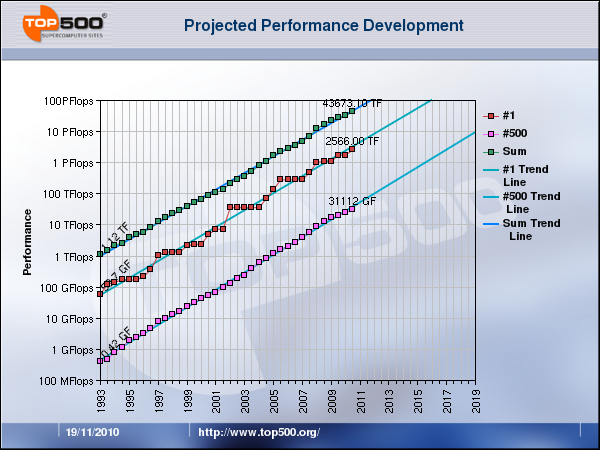
\includegraphics[scale=0.50]{./Sec_ET_ScienceCase/top500graph.png}
\caption{The Top500 past and projected performance (Image credit:
Prof. Dr. Hans W. Meuer ).} \label{fig:top500}
\end{figure*}

There are other factors limiting the possibility of taking full 
advantage of the modern CPU, such as internal bandwidth and 
storage speed. In other words memory and disk access speeds have 
failed to keep up with respect to the CPU. In fact, to reduce the 
impact due to these problems, different solutions have been 
introduced in processor and software design, examples of which
include out-of-order execution and caching and pre-fetching strategies. 
This also means that there is still a  big optimization margin 
on other computer components.

The key actions of the next decades can be summarised as follows:
\begin{itemize}
\item Chip-Level Multiprocessing (CMP)---increasing parallelism for enhanced 
performance (many-core architectures),
\item Special Purpose Hardware---embed important functions in
software and specialised chips inside the microprocessor itself,
\item Large Memory Subsystems---Memory access being the main bottleneck in
building many high-performing cores, it is important to have a large quantity of 
memory on-chip and close to the cores,
\item Microkernel---Microprocessors will need a sizable integrated 
intelligence, in order to coordinate all this complexity: assigning tasks to 
cores, powering up and powering down cores as needed, and, finally,
\item Virtualisation---Future microprocessors will need several levels of
virtualisation; virtualisation is needed to hide the complexity of the hardware
from the overlying software. Kernel and software should not have to deal with 
the intricacies of many cores, specialised execution hardware, multiple caches, 
reconfiguration and so on.
\end{itemize}

\etbox{r}{box:GPU}{GPU Computing for Coalescing Binaries}{
Tests carried out with NVIDIA C1060 (i.e.\ GT200) and NVIDIA C2050 
(i.e.\ the brand new Fermi GPU), are demonstrating how GPU 
implementation of the pipeline to search for coalescing binaries offers 
an average gain factor (normalised by price) of about 50 with respect to 
standard implementation using conventional CPUs~\cite{GPUarxive}.
This search involved the use of 30 matched filters per second.  The 
gain factor depends on the size of the data vector, assumed for
this search to be $2^{23}$ samples. Using shorter vectors it is 
possible to achieve even higher gains.  Performing the same test 
with the new NVIDIA Fermi GPU (i.e.\ the Tesla C2050),
one could increase the number of templates up to 120 templates per second. 
\\[0.25cm]
A preliminary fully multi-GPU implementation of the pipeline was 
reported at the E4 Workshop $2010$ in Bologna. This software implementation 
includes specifically an input data conditioning, post-Newtonian 
signal generator (up to 3.5 PN)~\cite{PGTesiPN} and a complete matched filtering 
procedure with coloured noise. This code offers an efficiency of 95\% using 4 
GPUs, bringing to an impressive result of proecessing about {\em 400 templates 
per second} with Tesla C2050 \cite{PGTesiMULTI}.
\\[0.25cm]
FFT algorithm is often the core of several data analysis and processing 
programs. Several benchmarks report a gain factor of  50-80, using GPU as
opposed to CPU architecture. This value has been renormalised by device prices.
Thus, we can state that using the already available many-core technologies the 
gain factor with respect to the standard single core architecture is, conservatively 
speaking, about 100. Obviously an exhaustive analysis of the gain factor needs 
to deal also with power consumption and other costs.}
%%%%%%%%%%%END BOX MANYCORE

As for the past 20 years, we can assume that during next decades these 
innovations will help to keep the Moore's law alive, which we 
can use to forecast the future computing power. 
Thus, if we consider the actual computing power of a typical CPU, Moore's
law predicts a gain factor of about 200 in 12 years and 700 in 14 years.
As general experimental proof of Moore's Law and computing evolution, we refer 
to {\em The Top500} project~\cite{website:top500}. Its goal is to generate, 
twice a year, a list of the 500 most powerful computers in the world. 
The Top500 ranking has always been a good overview of the actual technology
trends, and along the last ten to twenty years the list has showed an evident 
trend towards parallel and massively parallel systems. This trend has been 
confirmed by the appearance in the home computing system of superscalar and 
pipilened CPU firstly, and multi-core and many-core CPUs.
%At least up today, the Moore's Law behavior is experimentally proved also by 
%top500 performances graph shown in 
%figure~\ref{fig:top500}. As previously noted, the Linpack benchmark is used to 
%rank the system within the list. Thus, 
%the values reported in the graph can be considered a good estimation of the 
%real power (i.e.\ sustained performances) 
%of the 500 most powerful computer in the world. 

Figure~\ref{fig:top500} shows three different sequences.  The first one, 
labeled {\em Sum}, represents the combined computing power of all the 
500 supercomputers in the list. The second sequence, the one labeled \#1, 
is the power of the first ranked system. The last one, the sequence labeled 
\#500, is the computing power of the 500-th system in the list. 
If we consider the computing power of the last ranked system
in the list ten year ago, it is approximately 100 GFlops. 
Today, the 500th system, namely a Xeon Cluster, has a power of more 
the 10 TFlops. This gives a gain factor of about 100, consistent with 
the prediction of the Moore's first law. Though it may seem incredible, 
experimental data confirms that in the last ten years we had and increase 
of a factor 100 in computational speed.   

The actual Top500 list emphasises the following evolutionary characteristics: 
\begin{itemize}
\item Natural evolution from multi-core to many-core era (see Box \ref{box:GPU}),
\item Many-core architecture (i.e.\ GPU), together with multi-core X64 processors
is driving the technology,
\item Moore's Law is alive and still works well, and
\item Development of faster and more integrated interconnects is an obvious 
consequence of the increase in number nodes and cores.
\end{itemize}


To reiterate the aforementioned points one can cite the characteristics 
of the first ranked system on November 2010: the Tianhe-1A (see Box 
\ref{Tianhe1Abox}). This supercomputer is stationed at the National 
Supercomputer Center in Tianjin, it has achieved a performance level of 
2.57 petaflop/s. The system collects together both the trends: fast 
interconnection and many-cores. It is clear that a new programming 
paradigms and new algorithms are needed to get top performance from 
novel computing infrastructures.

As the complexity of a computational architecture grows, it is crucial
to design a computational system that is also flexible. Solutions can
be worked out only by gathering sufficient computing power and
the appropriate know-how.  Know-how and computing power must be 
collected and deployed in an efficient and appropriate manner, 
so that anyone is able to transparently access any needed information and resources. 
What we have just pointed out is the general idea of the grid or,
perhaps more precisely, of a computational grid environment. This new
approach to network computing is known by several names such as:
meta computing, scalable computing, global computing, internet computing,
and, more recently, peer-to-peer computing as discussed in Appendix
\ref{sec:gridcloudcomp}.

%%%%%%%%   box GRID computing

%\etbox{i}{gridcloudcomp}{Emerging technologies for distributed computing}{One 
%of the most famous
%definitions of the grid perfectly describes such design: "the grid is a
%flexible, secure, coordinated resource sharing among dynamic collections
%of individuals, institutions, and resources - what we refer to as
%virtual organizations." foster at al.~\cite{anatomy_grid}. 
%more precisely the grid can be thought as a distributed system, where 
%heterogeneous resources are geographically dispersed and connected by a 
%network.
%So grids represent a form of distributed computing facilities, where a 
%"super virtual computer" is composed by many interconnected computing 
%resources,
%like clusters, single workstations and traditional single super computers.
%The middleware (i.e.\ a collection of software libraries), like the operating 
%system in a pc, gives to the user all
%the necessary instruments to use the grid in a transparent and secure
%way, it provides uniformity through a standard set of interfaces to the
%underlying resources. It is a layer of software between the network and
%the applications that provides services such as identification,
%authentication, authorization, directories, and security. 
%A working example of what we briefly described is the Worldwide LHC Computing 
%Grid project (WLCG)~\cite{lcgwebsite}
%currently operates the world's largest scientific Grid, with over 
%140 computing centers in 34 countries contributing
%resources, including more than 10,000 CPUs and several Petabytes of storage. 
%Cloud computing goes a step further in the direction of separating the user 
%from the computing resources. This new computing paradigm represents also an 
%improvement in the direction 
%of the on-demand resource provisioning. Cloud computing generally means a 
%collection of technologies 
%enabling the final user to benefit of wide set of hardware and or software 
%remotely distributed.
%We can compares the Cloud with the electric power
%network: when we switch on a light, or we plug an
%electrical device into a wall socket, we are not aware from where the
%power comes from, and generally we do not care much about such details.
%Now we are thinking about a world in which computer power, storage and 
%software capabilities 
%are as easily accessible as the electric power. 
%Wen can try to briefly summarize the Cloud computing architecture as follow. 
%The final user simply uses a specific service provided by a customer 
%administrator.
%The administrator uses some interfaces to select a specific service (i.e.\ a 
%virtual server or 
%just some storage) and to administer the service (i.e.\ configure it, activate 
%or deactivate 
%the service, or maybe to ask for more computing power or storage). 
%The service provider is the one that physically owns the real server, and 
%it is the one in charge for providing some transparent interface to manage 
%the resources.
%There are up to now several examples of working cloud infrastructures : 
%Amazon Elastic Compute Cloud (EC2) (that allows users to rent and use virtual 
%server
%for the scalable deployment of applications), Amazon S3 (Simple Storage 
%Service, an online storage web service),
%Google App Engine (it is a platform for developing and hosting web applications
%in Google-managed data centers)
%}

%%%%%%%% end box GRID computing

Looking for high performances, one has also to deal with {\bf power 
consumption}. The power consumption of an HPC resource is a {\bf fundamental 
aspect} on computing facilities setup. This requires an optimization  in terms 
of efficiency, cost and resources reliability. 
%In order to stress how this is 
%today an extremely important and sensible theme, the Top500 has started to 
%collect data related to power consumption of the 500 most powerful computer in 
%the world.
To achieve greater performance per compute node, vendors have increased not just 
transistors and speed but consequently also the power density. Thus, a 
large-scale  high-performance computing system requires continual cooling in a 
large machine room, or even a new building in order to work properly. So to 
achieve greater performances one has  
to consider direct and indirect (i.e.\ cooling system) costs. We have to 
remember that the increase in failure rate of HPC systems is
directly related to their working temperature. 

%This second aspect is particularly important both because of cost, but mostly because 
%of its role in the software side. The software needs to be written in order to deal 
%with the intrinsic unreliability of the computing systems. So needs to be developed 
%following a different "paradigm", that is for example transparent run-time migration of tasks 
%between different computing resource, automatic management of recovery points, etc. etc.
Many-core systems seem to provide good performances also in terms of power 
consumption. In fact, making the assumption that The Tianhe-1A 2.5 PFlops system 
was built entirely with CPUs, it would have consumed more 
than 12 MW. Thanks to the use of GPUs in a heterogeneous computing 
environment, Tianhe-1A consumes only 4 MW, making it 3 times more 
power efficient. The most energy efficient supercomputers are based on: IBM 
BlueGene/Q Prototype with 1680 Mflop/watt, Fujitsu K-Computer at Riken with 829 
Mflop/watt, and QPace Clusters based on IBM PowerXCell 8i processor, up to 774 
Mflop/watt. Both the BlueGene/Q and the PowerXCell 8i are example of many-core 
systems.  This enforce the evidence that computing hardware architecture is moving 
towards the era of many-cores.



%%%%%%%%   box Tianhe-1A

\etbox{i}{Tianhe1Abox}{Tianhe-1A}{
This system is equipped with 29376 GB of memory, 
is based on Nvidia graphics processing units (GPUs) as well as Intel Xeon 5600 
series processors.
The Tianhe-1A is able to handle data at about twice the speed of InfiniBand, 
and the system 
has achieved a performance level of 2.57 petaflop/s essentially thanks to the 
the acceleration 
given by Nvidia Fermi GPU processors.
It is importaint to compare the power consumption of Tianhe-1A and Jaguar Cray 
XT5-HE, that is the second ranked system in top 500. In fact the
Jaguar use {\bf 5-10 MW} to achieve 1.7 PFlops while Tianhe-1A use {\bf 4 MW} 
to achieve 2.5 PFlops. {\bf This is a success of the many-core architecture 
providing 3-4 time more computing power per Watt!} 
}

%%%%%%%% end box Tianhe-1A


The above discussion, in particular processor speeds, is closely related with 
computational challenges faced by ET. In the ET era we can try to select some 
reference core algorithms and use the many-core, Moore's law forecast 
to predict the realistic computing power in 2025. These results can be 
used to understand the future capabilities and limitations in ET data analysis.
A fundamental point that distinguishes first and second generation gravitational 
wave detectors  with respect to ET is the nature of the experiment. ET has 
to possess enough sensitivity and computing power to achieve its main goal, 
namely to develop the field as a tool for obsrevational astronomy and cosmology. 
This means tha ET has to have the ability to perform real-time or on-time 
analysis. This will place severe demands on the computing infrastructure, 
requiring the handling together of two main data processing problems: 
detection and parameter reconstruction.
